\documentclass{standalone}
\usepackage{tikz}
\usetikzlibrary{patterns, positioning}
\usepackage[sfdefault]{ClearSans} %% option 'sfdefault' activates Clear Sans as the default text font
\usepackage[T1]{fontenc}

\begin{document}
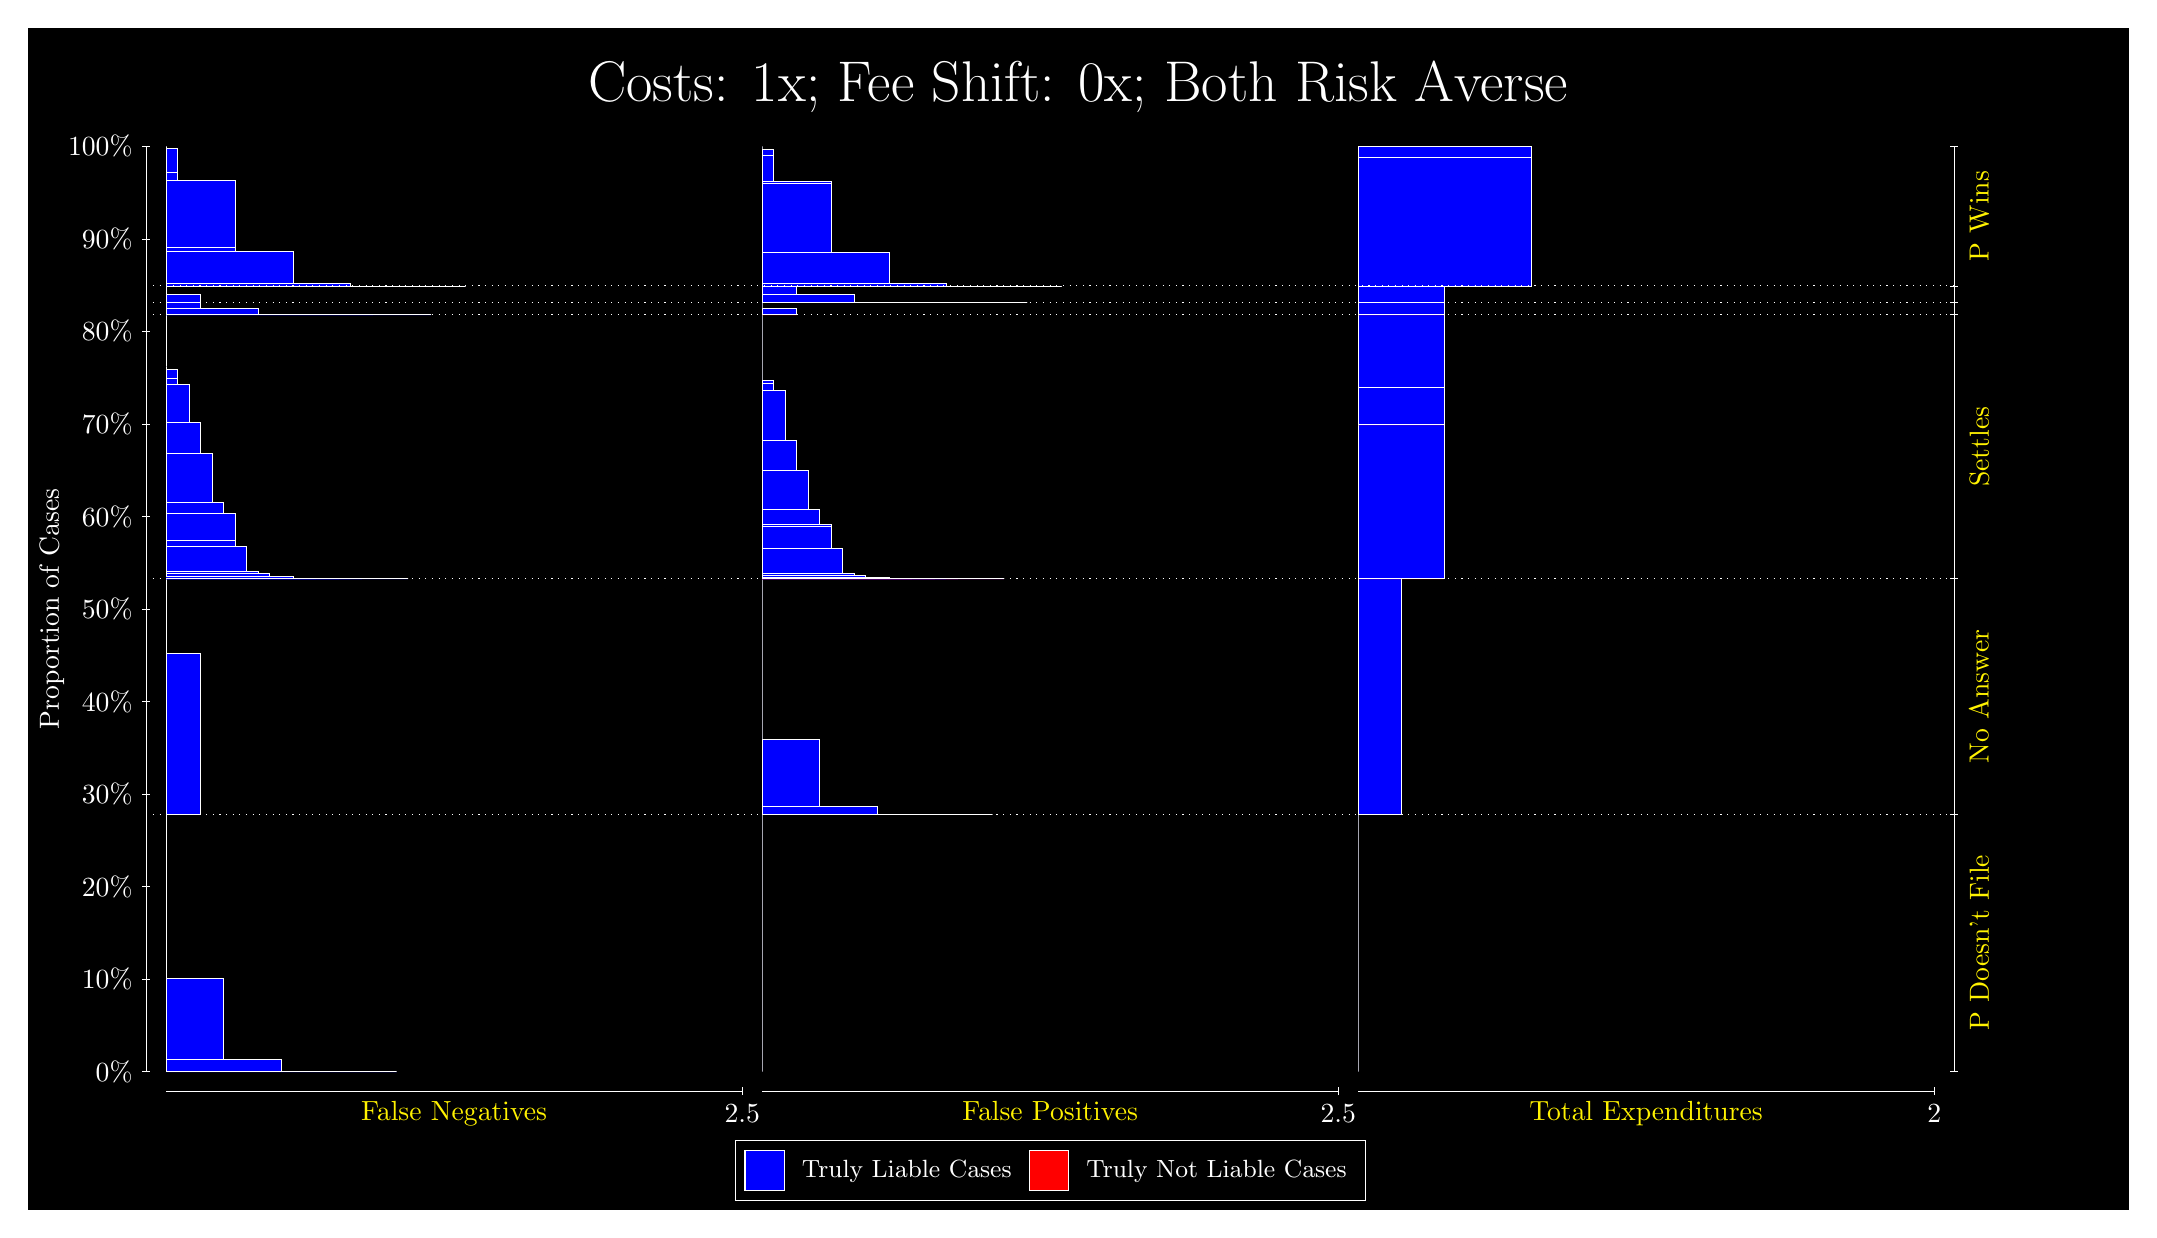
\begin{tikzpicture}
\draw[fill=black] (0,0) rectangle (26.667,15);
\draw[text=white] (0,13.5) rectangle (26.667,15) node[midway] {\huge Costs: 1x; Fee Shift: 0x; Both Risk Averse};
\draw[white, very thin] (1.5,1.75) -- (1.5,13.5);
\node[rotate=90, text=white, anchor=center] at (0.3, 7.625) {Proportion of Cases};
\draw[white, very thin] (1.45,1.75) -- (1.55,1.75);
\node[text=white, anchor=east] at (1.45, 1.75) {0\%};
\draw[white, very thin] (1.45,2.925) -- (1.55,2.925);
\node[text=white, anchor=east] at (1.45, 2.925) {10\%};
\draw[white, very thin] (1.45,4.1) -- (1.55,4.1);
\node[text=white, anchor=east] at (1.45, 4.1) {20\%};
\draw[white, very thin] (1.45,5.275) -- (1.55,5.275);
\node[text=white, anchor=east] at (1.45, 5.275) {30\%};
\draw[white, very thin] (1.45,6.45) -- (1.55,6.45);
\node[text=white, anchor=east] at (1.45, 6.45) {40\%};
\draw[white, very thin] (1.45,7.625) -- (1.55,7.625);
\node[text=white, anchor=east] at (1.45, 7.625) {50\%};
\draw[white, very thin] (1.45,8.8) -- (1.55,8.8);
\node[text=white, anchor=east] at (1.45, 8.8) {60\%};
\draw[white, very thin] (1.45,9.975) -- (1.55,9.975);
\node[text=white, anchor=east] at (1.45, 9.975) {70\%};
\draw[white, very thin] (1.45,11.15) -- (1.55,11.15);
\node[text=white, anchor=east] at (1.45, 11.15) {80\%};
\draw[white, very thin] (1.45,12.325) -- (1.55,12.325);
\node[text=white, anchor=east] at (1.45, 12.325) {90\%};
\draw[white, very thin] (1.45,13.5) -- (1.55,13.5);
\node[text=white, anchor=east] at (1.45, 13.5) {100\%};

\draw[white, very thin] (24.457,1.75) -- (24.457,13.5);
\draw[white, very thin] (24.407,1.75) -- (24.507,1.75);
\node[anchor=west] at (24.407, 1.75) {};
\draw[white, very thin] (24.407,5.019) -- (24.507,5.019);
\node[anchor=west] at (24.407, 5.019) {};
\draw[white, very thin] (24.407,8.0079) -- (24.507,8.0079);
\node[anchor=west] at (24.407, 8.0079) {};
\draw[white, very thin] (24.407,11.363) -- (24.507,11.363);
\node[anchor=west] at (24.407, 11.363) {};
\draw[white, very thin] (24.407,11.518) -- (24.507,11.518);
\node[anchor=west] at (24.407, 11.518) {};
\draw[white, very thin] (24.407,11.728) -- (24.507,11.728);
\node[anchor=west] at (24.407, 11.728) {};
\draw[white, very thin] (24.407,13.5) -- (24.507,13.5);
\node[anchor=west] at (24.407, 13.5) {};

\draw[white, very thin, fill=blue] (1.75,1.75) rectangle (4.6775,1.75);
\draw[white, very thin, fill=blue] (1.75,1.75) rectangle (3.9457,1.7513);
\draw[white, very thin, fill=blue] (1.75,1.7513) rectangle (3.2138,1.9056);
\draw[white, very thin, fill=blue] (1.75,1.9056) rectangle (2.4819,2.9325);
\draw[white, very thin, fill=red] (1.75,2.9325) rectangle (1.75,2.9325);
\draw[white, very thin, fill=blue] (1.75,2.9325) rectangle (1.75,5.019);
\draw[white, very thin, fill=blue] (1.75,5.019) rectangle (2.1891,7.0574);
\draw[white, very thin, fill=red] (1.75,7.0574) rectangle (1.75,7.0574);
\draw[white, very thin, fill=blue] (1.75,7.0574) rectangle (1.75,8.0079);
\draw[white, very thin, fill=blue] (1.75,8.0079) rectangle (4.8239,8.0079);
\draw[white, very thin, fill=blue] (1.75,8.0079) rectangle (4.2384,8.0079);
\draw[white, very thin, fill=blue] (1.75,8.0079) rectangle (4.092,8.0079);
\draw[white, very thin, fill=blue] (1.75,8.0079) rectangle (3.9457,8.0079);
\draw[white, very thin, fill=blue] (1.75,8.0079) rectangle (3.6529,8.0079);
\draw[white, very thin, fill=blue] (1.75,8.0079) rectangle (3.5065,8.0168);
\draw[white, very thin, fill=blue] (1.75,8.0168) rectangle (3.3602,8.0361);
\draw[white, very thin, fill=blue] (1.75,8.0361) rectangle (3.2138,8.0366);
\draw[white, very thin, fill=blue] (1.75,8.0366) rectangle (3.0674,8.0737);
\draw[white, very thin, fill=blue] (1.75,8.0737) rectangle (2.921,8.0984);
\draw[white, very thin, fill=blue] (1.75,8.0984) rectangle (2.7746,8.4227);
\draw[white, very thin, fill=blue] (1.75,8.4227) rectangle (2.6283,8.4973);
\draw[white, very thin, fill=blue] (1.75,8.4973) rectangle (2.6283,8.8425);
\draw[white, very thin, fill=blue] (1.75,8.8425) rectangle (2.4819,8.9734);
\draw[white, very thin, fill=blue] (1.75,8.9734) rectangle (2.3355,9.6043);
\draw[white, very thin, fill=blue] (1.75,9.6043) rectangle (2.1891,9.9903);
\draw[white, very thin, fill=blue] (1.75,9.9903) rectangle (2.0428,10.475);
\draw[white, very thin, fill=blue] (1.75,10.475) rectangle (1.8964,10.557);
\draw[white, very thin, fill=blue] (1.75,10.557) rectangle (1.8964,10.67);
\draw[white, very thin, fill=blue] (1.75,10.67) rectangle (1.75,10.702);
\draw[white, very thin, fill=red] (1.75,10.702) rectangle (1.75,10.702);
\draw[white, very thin, fill=blue] (1.75,10.702) rectangle (1.75,11.363);
\draw[white, very thin, fill=blue] (1.75,11.363) rectangle (5.1167,11.363);
\draw[white, very thin, fill=blue] (1.75,11.363) rectangle (4.3848,11.363);
\draw[white, very thin, fill=blue] (1.75,11.363) rectangle (3.6529,11.365);
\draw[white, very thin, fill=blue] (1.75,11.365) rectangle (2.921,11.443);
\draw[white, very thin, fill=blue] (1.75,11.443) rectangle (2.1891,11.518);
\draw[white, very thin, fill=red] (1.75,11.518) rectangle (1.75,11.518);
\draw[white, very thin, fill=blue] (1.75,11.518) rectangle (2.1891,11.619);
\draw[white, very thin, fill=red] (1.75,11.619) rectangle (1.75,11.619);
\draw[white, very thin, fill=blue] (1.75,11.619) rectangle (1.75,11.728);
\draw[white, very thin, fill=blue] (1.75,11.728) rectangle (5.5558,11.728);
\draw[white, very thin, fill=blue] (1.75,11.728) rectangle (4.8239,11.728);
\draw[white, very thin, fill=blue] (1.75,11.728) rectangle (4.092,11.76);
\draw[white, very thin, fill=blue] (1.75,11.76) rectangle (3.3602,12.166);
\draw[white, very thin, fill=blue] (1.75,12.166) rectangle (2.6283,12.222);
\draw[white, very thin, fill=blue] (1.75,12.222) rectangle (2.6283,13.075);
\draw[white, very thin, fill=blue] (1.75,13.075) rectangle (1.8964,13.165);
\draw[white, very thin, fill=blue] (1.75,13.165) rectangle (1.8964,13.47);
\draw[white, very thin, fill=red] (1.75,13.47) rectangle (1.75,13.47);
\draw[white, very thin, fill=blue] (1.75,13.47) rectangle (1.75,13.5);
\draw[white, very thin, fill=red] (9.3189,1.75) rectangle (9.3189,1.75);
\draw[white, very thin, fill=blue] (9.3189,1.75) rectangle (9.3189,5.019);
\draw[white, very thin, fill=red] (9.3189,5.019) rectangle (12.246,5.019);
\draw[white, very thin, fill=blue] (9.3189,5.019) rectangle (12.246,5.019);
\draw[white, very thin, fill=blue] (9.3189,5.019) rectangle (11.515,5.0193);
\draw[white, very thin, fill=blue] (9.3189,5.0193) rectangle (10.783,5.119);
\draw[white, very thin, fill=blue] (9.3189,5.119) rectangle (10.051,5.9695);
\draw[white, very thin, fill=blue] (9.3189,5.9695) rectangle (9.3189,8.0079);
\draw[white, very thin, fill=red] (9.3189,8.0079) rectangle (12.393,8.0079);
\draw[white, very thin, fill=blue] (9.3189,8.0079) rectangle (12.393,8.0079);
\draw[white, very thin, fill=red] (9.3189,8.0079) rectangle (11.807,8.0079);
\draw[white, very thin, fill=blue] (9.3189,8.0079) rectangle (11.807,8.0079);
\draw[white, very thin, fill=blue] (9.3189,8.0079) rectangle (11.661,8.0079);
\draw[white, very thin, fill=red] (9.3189,8.0079) rectangle (11.515,8.0079);
\draw[white, very thin, fill=blue] (9.3189,8.0079) rectangle (11.515,8.0079);
\draw[white, very thin, fill=red] (9.3189,8.0079) rectangle (11.222,8.0079);
\draw[white, very thin, fill=blue] (9.3189,8.0079) rectangle (11.222,8.0079);
\draw[white, very thin, fill=blue] (9.3189,8.0079) rectangle (11.075,8.0168);
\draw[white, very thin, fill=blue] (9.3189,8.0168) rectangle (10.929,8.0324);
\draw[white, very thin, fill=red] (9.3189,8.0324) rectangle (10.929,8.0324);
\draw[white, very thin, fill=blue] (9.3189,8.0324) rectangle (10.929,8.0325);
\draw[white, very thin, fill=blue] (9.3189,8.0325) rectangle (10.783,8.0329);
\draw[white, very thin, fill=red] (9.3189,8.0329) rectangle (10.636,8.0329);
\draw[white, very thin, fill=blue] (9.3189,8.0329) rectangle (10.636,8.058);
\draw[white, very thin, fill=blue] (9.3189,8.058) rectangle (10.49,8.0831);
\draw[white, very thin, fill=blue] (9.3189,8.0831) rectangle (10.344,8.4007);
\draw[white, very thin, fill=blue] (9.3189,8.4007) rectangle (10.197,8.6688);
\draw[white, very thin, fill=blue] (9.3189,8.6688) rectangle (10.197,8.7012);
\draw[white, very thin, fill=red] (9.3189,8.7012) rectangle (10.051,8.7012);
\draw[white, very thin, fill=blue] (9.3189,8.7012) rectangle (10.051,8.8962);
\draw[white, very thin, fill=blue] (9.3189,8.8962) rectangle (9.9044,9.381);
\draw[white, very thin, fill=blue] (9.3189,9.381) rectangle (9.758,9.767);
\draw[white, very thin, fill=blue] (9.3189,9.767) rectangle (9.6116,10.398);
\draw[white, very thin, fill=blue] (9.3189,10.398) rectangle (9.4652,10.485);
\draw[white, very thin, fill=blue] (9.3189,10.485) rectangle (9.4652,10.529);
\draw[white, very thin, fill=blue] (9.3189,10.529) rectangle (9.3189,11.363);
\draw[white, very thin, fill=red] (9.3189,11.363) rectangle (9.758,11.363);
\draw[white, very thin, fill=blue] (9.3189,11.363) rectangle (9.758,11.438);
\draw[white, very thin, fill=blue] (9.3189,11.438) rectangle (9.3189,11.518);
\draw[white, very thin, fill=red] (9.3189,11.518) rectangle (12.686,11.518);
\draw[white, very thin, fill=blue] (9.3189,11.518) rectangle (12.686,11.518);
\draw[white, very thin, fill=blue] (9.3189,11.518) rectangle (11.954,11.518);
\draw[white, very thin, fill=blue] (9.3189,11.518) rectangle (11.222,11.52);
\draw[white, very thin, fill=blue] (9.3189,11.52) rectangle (10.49,11.626);
\draw[white, very thin, fill=blue] (9.3189,11.626) rectangle (9.758,11.728);
\draw[white, very thin, fill=red] (9.3189,11.728) rectangle (13.125,11.728);
\draw[white, very thin, fill=blue] (9.3189,11.728) rectangle (13.125,11.728);
\draw[white, very thin, fill=red] (9.3189,11.728) rectangle (12.393,11.728);
\draw[white, very thin, fill=blue] (9.3189,11.728) rectangle (12.393,11.728);
\draw[white, very thin, fill=red] (9.3189,11.728) rectangle (11.661,11.728);
\draw[white, very thin, fill=blue] (9.3189,11.728) rectangle (11.661,11.758);
\draw[white, very thin, fill=red] (9.3189,11.758) rectangle (10.929,11.758);
\draw[white, very thin, fill=blue] (9.3189,11.758) rectangle (10.929,12.153);
\draw[white, very thin, fill=blue] (9.3189,12.153) rectangle (10.197,13.028);
\draw[white, very thin, fill=red] (9.3189,13.028) rectangle (10.197,13.028);
\draw[white, very thin, fill=blue] (9.3189,13.028) rectangle (10.197,13.062);
\draw[white, very thin, fill=blue] (9.3189,13.062) rectangle (9.4652,13.386);
\draw[white, very thin, fill=blue] (9.3189,13.386) rectangle (9.4652,13.468);
\draw[white, very thin, fill=blue] (9.3189,13.468) rectangle (9.3189,13.5);
\draw[white, very thin, fill=red] (16.888,1.75) rectangle (16.888,1.75);
\draw[white, very thin, fill=blue] (16.888,1.75) rectangle (16.888,5.019);
\draw[white, very thin, fill=red] (16.888,5.019) rectangle (17.437,5.019);
\draw[white, very thin, fill=blue] (16.888,5.019) rectangle (17.437,8.0079);
\draw[white, very thin, fill=red] (16.888,8.0079) rectangle (17.986,8.0079);
\draw[white, very thin, fill=blue] (16.888,8.0079) rectangle (17.986,9.967);
\draw[white, very thin, fill=red] (16.888,9.967) rectangle (17.986,9.967);
\draw[white, very thin, fill=blue] (16.888,9.967) rectangle (17.986,10.444);
\draw[white, very thin, fill=red] (16.888,10.444) rectangle (17.986,10.444);
\draw[white, very thin, fill=blue] (16.888,10.444) rectangle (17.986,11.363);
\draw[white, very thin, fill=red] (16.888,11.363) rectangle (17.986,11.363);
\draw[white, very thin, fill=blue] (16.888,11.363) rectangle (17.986,11.518);
\draw[white, very thin, fill=red] (16.888,11.518) rectangle (17.986,11.518);
\draw[white, very thin, fill=blue] (16.888,11.518) rectangle (17.986,11.728);
\draw[white, very thin, fill=red] (16.888,11.728) rectangle (19.083,11.728);
\draw[white, very thin, fill=blue] (16.888,11.728) rectangle (19.083,13.364);
\draw[white, very thin, fill=red] (16.888,13.364) rectangle (19.083,13.364);
\draw[white, very thin, fill=blue] (16.888,13.364) rectangle (19.083,13.5);
\draw[white, dotted] (1.5,5.019) -- (24.457,5.019);
\draw[white, dotted] (1.5,8.0079) -- (24.457,8.0079);
\draw[white, dotted] (1.5,11.363) -- (24.457,11.363);
\draw[white, dotted] (1.5,11.518) -- (24.457,11.518);
\draw[white, dotted] (1.5,11.728) -- (24.457,11.728);
\draw[white, very thin] (1.75,1.5) -- (9.0689,1.5);
\node[text=yellow, anchor=north] at (5.4094, 1.5) {False Negatives};
\draw[white, very thin] (9.0689,1.45) -- (9.0689,1.55);
\node[text=white, anchor=north] at (9.0689, 1.45) {2.5};

\draw[white, very thin] (9.3189,1.5) -- (16.638,1.5);
\node[text=yellow, anchor=north] at (12.978, 1.5) {False Positives};
\draw[white, very thin] (16.638,1.45) -- (16.638,1.55);
\node[text=white, anchor=north] at (16.638, 1.45) {2.5};

\draw[white, very thin] (16.888,1.5) -- (24.207,1.5);
\node[text=yellow, anchor=north] at (20.547, 1.5) {Total Expenditures};
\draw[white, very thin] (24.207,1.45) -- (24.207,1.55);
\node[text=white, anchor=north] at (24.207, 1.45) {2};

\node[text=yellow, centered, rotate=90] at (24.777, 3.3845) {P Doesn't File};
\node[text=yellow, centered, rotate=90] at (24.777, 6.5135) {No Answer};
\node[text=yellow, centered, rotate=90] at (24.777, 9.6856) {Settles};


\node[text=yellow, centered, rotate=90] at (24.777, 12.614) {P Wins};

\draw (12.978300999999998,1.5) node[draw=none] (baseCoordinate) {};
\begin{scope}[align=center]
        \matrix[scale=0.5, draw=white, below=0.5cm of baseCoordinate, nodes={draw}, column sep=0.1cm]{
            \node[rectangle, draw, minimum width=0.5cm, minimum height=0.5cm, fill=blue] {}; &
            \node[draw=none, font=\small, text=white] (B) {Truly Liable Cases}; &
            \node[rectangle, draw, minimum width=0.5cm, minimum height=0.5cm, fill=red] {}; &
            \node[draw=none, font=\small, text=white] (B) {Truly Not Liable Cases}; \\
            };
\end{scope}

\end{tikzpicture}
\end{document}